\documentclass[onecolumn,notitlepage,letterpaper,aps,pra,12pt]{article}
\usepackage[utf8]{inputenc}
\usepackage[spanish, es-tabla]{babel}
\usepackage[T1]{fontenc}
\usepackage[version=3]{mhchem}
\usepackage{titlesec}
\usepackage{enumitem}
\usepackage{pdfpages}
\usepackage{setspace}  
\usepackage{lmodern}
\usepackage{beamerarticle}
%\usepackage{multicol}
\usepackage{fancyhdr}
\setlength{\headheight}{15.13202pt}
\usepackage{graphics}
\usepackage{graphicx}
\usepackage{microtype} 
%\usepackage{natbib}
\usepackage[backend=bibtex,style=phys,natbib=true]{biblatex}

% Redefinimos el formato de los números en la bibliografía
\DeclareFieldFormat{labelnumberwidth}{[#1]} % Cambia superíndices a corchetes
\setlength{\biblabelsep}{0.5em} % Espacio entre el número y la referencia

\addbibresource{references.bib}
\DeclareFieldFormat[article]{title}{#1}
\usepackage{subfigure}
\usepackage{svg}
\usepackage{multirow} 
\usepackage{amssymb, amsmath, amsbsy} % simbolitos
\numberwithin{equation}{section}
\usepackage{upgreek} % para poner letras griegas sin cursiva
\usepackage{cancel} % para tachar
\usepackage{mathdots} % para el comando \iddots
\usepackage{mathrsfs} % para formato de letra
\usepackage{geometry}
\geometry{
	a4paper,
	total={150mm,257mm},
	left=20mm,
	top=20mm,
}
%\titleformat*{\section}{\bfseries\large}
%\titleformat*{\subsection}{\bfseries\normalsize}
\titleformat*{\section}{\normalfont\Large\bfseries\color{darkgray}}
\titleformat*{\subsection}{\normalfont\large\bfseries\color{gray}}
\titleformat*{\subsubsection}{\normalfont\normalsize\bfseries\color{blue}}
\usepackage{fancyhdr}
\pagestyle{fancy}
\rfoot{PROPUESTA DE INVESTIGACIÓN}
\renewcommand{\headrulewidth}{3pt}
\usepackage{tabularx}
\usepackage{supertabular}
\usepackage{vmargin}
\usepackage{mathtools} 
\usepackage{amsfonts}
\usepackage{float}
\usepackage{parskip}
\usepackage{times}
\usepackage{calligra}
\usepackage{latexsym}
\usepackage{booktabs}
\usepackage{tabulary}
\usepackage{caption}
\usepackage{url}
\spanishdecimal{.}
\usepackage{ragged2e}
%\bibliographystyle{unsrt}
\usepackage[usenames,dvipsnames]{pstricks}
\usepackage{epsfig}
\usepackage{pst-grad} % For gradients
\usepackage{pst-plot} % For axes
\usepackage{colortbl}
\usepackage{hyperref}
\usepackage{latexsym}
\usepackage{xcolor}
\usepackage{fancyhdr}
\usepackage{balance}
\usepackage{float}
\usepackage{bbold}
\usepackage[normalem]{ulem}
\usepackage{physics}
\usepackage{derivative}
\usepackage{tcolorbox}
\usepackage{amssymb}

% New commands
\newcommand{\miguel}[1]{{\color{magenta}#1}} 
\newcommand{\ricardo}[1]{{\color{red}#1}} 

%%%%%%%%%%%%%%%%%%%%%%%%%%%%%%
%%%%%%%%%%%%%%%%%%%%%%%%%%%%%%
\begin{document} 
%%%%%%%%%%%%%%%%%%%%%%%%%%%%%%
%%%%%%%%%%%%%%%%%%%%%%%%%%%%%%

\clearpage
\thispagestyle{empty}

%%%%%%%%%%%%%%%%%%%%%%%%%%%%%%
%%%%%%%%%%%%%%%%%%%%%%%%%%%%%%
\begin{titlepage}
\centering
\begin{figure}
    \centering
    
\includegraphics[width=4.5 in]{Images/uam.png}
\end{figure}

\vspace{1cm}

{\LARGE \rule{15cm}{1.0mm}  \par}

\centering
\vspace{0.45cm}

{\LARGE División de Ciencias Básicas e Ingeniería}

\centering
\vspace{0.45cm}

{\LARGE Posgrado en Ciencias (Física)}

\centering
\vspace{0.45cm}

{\LARGE Propuesta de Investigación Doctoral}

\vspace{0.25cm}

{\Huge \textbf{Fenómenos fuera de equilibrio en sistemas multimodo espín-bosón}}

\vspace{0.45cm}
{\large Propuesto por: {\bf M. en C. Ricardo Herrera Romero} \par}

\vspace{0.45cm}
{\large Matrícula: {\bf 2221801209} \par}

\vspace{0.45cm}
{\large Para sustentar el {\bf Examen Predoctoral} \par}

\vspace{0.45cm}
{\large Asesor: \textbf{Dr. Miguel Angel Bastarrachea Magnani}  \par}

\vspace{1cm}
\rule{5cm}{0.3mm}

\vspace{0.45cm}
{\large Coordinador: \textbf{Dr. Orlando Guzmán López}  \par}

{\LARGE \rule{15cm}{1.0mm}  \par}

\vspace{0.4cm}

{\large 18 de marzo de 2025 \par}
\vspace{0.1cm}
{\large Iztapalapa, Ciudad de México \par}
\end{titlepage}

%%%%%%%%%%%%%%%%%%%%%%%%%%%%%%
%%%%%%%%%%%%%%%%%%%%%%%%%%%%%%
\clearpage
\tableofcontents
\clearpage
\newpage
%%%%%%%%%%%%%%%%%%%%%%%%%%%%%%
%%%%%%%%%%%%%%%%%%%%%%%%%%%%%%

%%%%%%%%%%%%%%%%%%%%%%%%%%%%%%
%%%%%%%%%%%%%%%%%%%%%%%%%%%%%%
%\section*{Resumen}
%%%%%%%%%%%%%%%%%%%%%%%%%%%%%%
%%%%%%%%%%%%%%%%%%%%%%%%%%%%%%

%%%%%%%%%%%%%%%%%%%%%%%%%%%%%%
%%%%%%%%%%%%%%%%%%%%%%%%%%%%%%

%%%%%%%%%%%%%%%%%%%%%%%%%%%%%%
%%%%%%%%%%%%%%%%%%%%%%%%%%%%%%
\section{Introducción}
%%%%%%%%%%%%%%%%%%%%%%%%%%%%%%
%%%%%%%%%%%%%%%%%%%%%%%%%%%%%%



En las últimas décadas, los sistemas de interacción spin-bosón se han convertido en un área central en la física~\cite{haroche2006} CITAR. El desarrollo de plataformas experimentales como cavidades y circuitos en electrodinámica cuántica (\textit{Quantum Electrodynamics} o QED)~\cite{Blais2021,Clerk2020}, sistemas de átomos fríos~\cite{Mekhov2012}, trampas ópticas~\cite{Yuanjie2021} o semiconductores acoplados a microcavidades~\cite{Schneider2018}, han permitido explorar el acoplamiento controlado entre excitaciones bosónicas (fotones) y sistemas discretos de dos niveles (qubits o átomos de espin $1/2$). %Más allá de su interés en óptica cuántica, estas arquitecturas  funcionan como simuladores cuánticos de fenómenos colectivos~\cite{caballero2016}.

Los sistemas abiertos y fuertemente acoplados, donde la interacción entre spin-bosón es comparable o mayor que las frecuencias propias del sistema— han cobrado relevancia experimental en los últimos años~\cite{Grifoni1999,ZhangHou2015,Burger2022,Fazio2025}. La disipación y el bombeo generan estados de equilibrio dinámico con coherencia colectiva, que reflejan nuevas formas de comportamiento organizado~\cite{Sieberer2016,Halati2020,Chelpanova2025}. El interés se centra, por tanto, en la competencia entre coherencia, interacción spin-bosón y disipación, lo que permite comprender y controlar el comportamiento colectivo en regímenes de acoplamiento intenso~\cite{subasi2012,FornDiaz2019,Kirton2018,LeBoite2020,roses2020}.

Es en este marco conceptual modelos de spin-bosón como Rabi y Dicke adquieren relevancia, permitiendo analizar la dinámica de bombeo y disipación en estos sistemas~\cite{henriet2014,hwang2018,DiBello2024-2,Nagy10,Klinder15}. La propuesta de tesis doctoral se enmarca en esta dirección, con un enfoque sistemático y progresivo: comenzar con el modelo de Rabi abierto y avanzar hacia el modelo de Dicke abierto, incorporando tanto múltiples qubits como múltiples modos bosó\-nicos, para explorar la interacción colectiva y multimodal en presencia de bombeo y disipación.


%%%%%%%%%%%%%%%%%%%%%%%%%%%%%%
%%%%%%%%%%%%%%%%%%%%%%%%%%%%%%
\subsection{Modelos de interacción espín-bosón}
%%%%%%%%%%%%%%%%%%%%%%%%%%%%%%
%%%%%%%%%%%%%%%%%%%%%%%%%%%%%%

El estudio de la interacción entre la radiación y sistemas de dos niveles (espín–bosón) tiene su origen en el modelo de Rabi, propuesto para describir el acoplamiento coherente entre un átomo y un modo del campo electromagnético~\cite{rabi1936}. Su Hamiltoniano,

\begin{gather}\label{Hamiltoniano de Rabi}
    \hat{H}_{\text{Rabi}} = \omega\hat{a}^{\dagger}\hat{a} + \frac{\omega_{0}}{2}\hat{\sigma}_{z} + g\left( \hat{\sigma}_{+} + \hat{\sigma}_{-} \right)\left( \hat{a}^{\dagger} + \hat{a} \right),
\end{gather}

describe la energía del campo (frecuencia $\omega$) y del átomo (frecuencia $\omega_{0}$). El parámetro $g$ caracteriza el acoplamiento entre ambos, mientras que los términos rotantes $(\hat{\sigma}_{-}\hat{a} + \hat{\sigma}_{+}\hat{a}^{\dagger})$ representan procesos que conservan el número de excitaciones: la emisión o absorción de un fotón acompañada de la desexcitación o excitación atómica.

El modelo de Jaynes–Cummings~\cite{Jaynes1963} se obtiene aplicando la aproximación de onda rotante (RWA), que descarta los términos contra–rotantes $(\hat{\sigma}_{+}\hat{a}^{\dagger} + \hat{\sigma}_{-}\hat{a})$ válidos sólo en el régimen de acoplamiento débil $(g \ll \omega,\omega_{0})$. Esta aproximación permitió una descripción analítica del intercambio coherente de energía entre el átomo y el campo~\cite{wallraff2004,Schoelkopf2008,devoret2013}. Sin embargo, los avances experimentales han permitido acceder a los regímenes ultrastrong $(g/\omega \gtrsim 0.1)$ y deep strong $(g/\omega \gtrsim 1)$, donde la RWA deja de ser válida~\cite{FornDiaz2019,Yoshihara2017}, y se requiere el modelo de Rabi completo.

Un paso natural para extender el modelo a sistemas multiqubit consiste en analizar el caso de dos qubits acoplados colectivamente a un modo del campo, descrito por:

\begin{gather}
    \hat{H} = \omega\hat{a}^{\dagger}\hat{a} + \frac{\omega_{01}}{2}\hat{\sigma}_{z}^{1} + \frac{\omega_{02}}{2}\hat{\sigma}_{z}^{2} + \frac{g}{2}\left(\hat{\sigma}_{x}^{1}+\hat{\sigma}_{x}^{2}\right)(\hat{a}^{\dagger}+\hat{a}).
\end{gather}

Mediante los coeficientes de Clebsch–Gordan, los estados de los dos qubits pueden representarse en la base de espín total \( |J,M\rangle \), que se descompone en un subespacio simétrico triplete (\(J=1\)) y un singlete antisimétrico (\(J=0\)). Si las frecuencias atómicas son similares \(\omega_{01} \approx \omega_{02}\), el sistema es invariante bajo permutación y puede describirse dentro del subespacio simétrico \(J=1\). En esta representación, los operadores individuales se reemplazan por operadores colectivos \(\hat{J}_{\alpha}=\tfrac{1}{2}(\hat{\sigma}_{\alpha}^{1}+\hat{\sigma}_{\alpha}^{2})\), obteniendo el Hamiltoniano efectivo:

\begin{gather}\label{Hamiltoniano de Rabi dos qubits con interacciones}
    \hat{H} = \omega \hat{a}^{\dagger}\hat{a} + \omega_{0} \hat{J}_{z} + g \hat{J}_{x} (\hat{a}^{\dagger} + \hat{a}) + \eta_{x} \hat{J}_{x}^{2} + \eta_{z} \hat{J}_{z}^{2}.
\end{gather}

Los términos \(\eta_{z}\hat{J}_{z}^{2}\) y \(\eta_{x}\hat{J}_{x}^{2}\) introducen interacciones efectivas entre los qubits. El primero corresponde a un acoplamiento tipo Ising, que modula la energía según la alineación de los momentos atómicos; el segundo, de tipo XY, describe el intercambio coherente de excitaciones responsable de la correlación dinámica entre los emisores.

La generalización a un número arbitrario de átomos lleva al modelo de Dicke~\cite{Dicke54}, que describe la interacción colectiva entre $N$ átomos idénticos y un modo del campo electromagnético:

\begin{gather}
    \hat{H}_{\text{D}} = \omega\hat{a}^{\dagger}\hat{a} + \sum_{j=1}^{N}\left[ \frac{\omega_{0}}{2}\hat{\sigma}_{z}^{j} + \frac{g}{\sqrt{N}}\hat{\sigma}_{x}^{j}\left(\hat{a}^{\dagger} + \hat{a}\right) \right].
\end{gather}

Bajo la aproximación de onda larga~\cite{Dicke54}, todos los átomos experimentan el mismo campo, y el sistema puede describirse mediante los operadores de pseudospín colectivos \(\hat{J}_{\mu} = \frac{1}{2}\sum_{i=1}^{N}\hat{\sigma}_{\mu}^{i}\), lo que conduce a la forma compacta:

\begin{gather}\label{Dicke colectivo}
    \hat{H}_{\text{D}} = \omega\hat{a}^{\dagger}\hat{a} + \omega_{0}\hat{J}_{z} + \frac{2g}{\sqrt{N}}\hat{J}_{x}\left( \hat{a}^{\dagger} + \hat{a} \right).
\end{gather}

Este modelo predice fenómenos críticos como las transiciones de fase cuánticas (QPT) y las transiciones de fase cuánticas de estados excitados (ESQPT)~\cite{Hepp73,wang1973,hioe1973,Sachdev99,Larson17}. Cuando el acoplamiento luz-materia supera un valor crítico, el sistema pasa de un estado normal (sin fotones) a un estado superradiante caracterizado por emisión coherente colectiva~\cite{gross1982}. El modelo de Dicke ha sido implementado experimentalmente en diversas plataformas, como circuitos superconductores~\cite{Blais04,Casanova10} y cavidades ópticas con transiciones Raman~\cite{Baden14,Nagy10}, y se ha consolidado como un marco relevante en información cuántica~\cite{Garraway2011,Kirton2018,LeBoite2020}.



La inclusión de interacciones entre los átomos en el modelo de Dicke permite explorar nuevas fases y modificar los puntos críticos del sistema. En mi trabajo de maestría, estudié un modelo de Dicke anisotrópico con interacciones colectivas entre emisores, analizando su diagrama de fases y la aparición de QPT y ESQPT~\cite{Herrera2022}. Posteriormente identifiqué modos de fase y amplitud, relacionando anisotropía y criticidad en sistemas luz-materia fuertemente acoplados~\cite{herrera2024}. El Hamiltoniano correspondiente es:

\begin{gather}\label{Hamiltoniano de Dicke con interacciones}
    \hat{H}_{\text{I}} = \omega\hat{a}^{\dagger}\hat{a} + \omega_{0}\hat{J}_{z} + \frac{\gamma}{\sqrt{N}}\left[ \hat{a}\hat{J}_{+} + \hat{a}^{\dagger}\hat{J}_{-} + \xi\left( \hat{a}\hat{J}_{-} + \hat{a}^{\dagger}\hat{J}_{+} \right)  \right] + \frac{1}{N}\sum_{i=x,y,z} \eta_{i}\hat{J}_{i}^{2}.
\end{gather}

Los términos rotantes $(\hat{a}\hat{J}_{+}, \hat{a}^{\dagger}\hat{J}_{-})$ y contra–rotantes $(\hat{a}\hat{J}_{-}, \hat{a}^{\dagger}\hat{J}_{+})$ son modulados por el parámetro anisotrópico $\xi$, mientras que los términos $\eta_{i}$ cuantifican la interacción entre emisores.

Recientemente, se han propuesto extensiones multimodo del modelo de Dicke~\cite{tolkunov2007,fiorelli2020,carollo2021}, donde múltiples modos del campo electromagnético interactúan con los átomos:

\begin{gather}
        \hat{H}_{\text{Multimodo}} = \sum_{k}\left(\omega_{k}\hat{a}^{\dagger}_{k}\hat{a}_{k} + \sum_{j=1}^{N}\left[ \frac{\omega_{0}}{2}\hat{\sigma}_{z}^{j} + \sum_{k}\frac{g_{k}}{\sqrt{N}}\hat{\sigma}_{x}^{j}\left(\hat{a}^{\dagger}_{k} + \hat{a}_{k}\right) \right]\right).
\end{gather}

Estos sistemas presentan fenómenos como competencia entre modos, fases no convencionales y efectos de desorden~\cite{rotondo2015,kipf2014,vojta2013,das2024}, con implicaciones en el almacenamiento cuántico y redes neuronales cuánticas~\cite{maniscalco2006,fiorelli2020,marsch2021}.

De manera paralela, la física de los llamados “átomos gigantes” ha emergido como una extensión natural de estos modelos. En ellos, un solo emisor se acopla a un campo en múltiples puntos espaciales, generando retardos, interferencias y efectos no markovianos~\cite{Andersson2019,gonzalez2021-2,cai2021,yu2025}. Su tamaño efectivo, comparable con la longitud de onda del campo, rompe la aproximación dipolar y permite fenómenos como estados ligados dentro y fuera del continuo (BIC y BOC)~\cite{gonzalez2025,guo2020}. Experimentalmente, estos sistemas se implementan en circuitos superconductores donde qubits tipo transmon se acoplan en múltiples puntos de una guía de onda~\cite{Kannan2020}.

Los átomos gigantes constituyen un puente entre los modelos multiqubit y multimodo, donde la estructura espacial y temporal del acoplamiento genera nuevas dinámicas colectivas. Su estudio abre oportunidades para comprender efectos de memoria cuántica y explorar arquitecturas de simulación cuántica con acoplamientos no markovianos. Esta línea se alinea con el enfoque progresivo de esta tesis: analizar cómo la inclusión de grados de libertad multiqubit y multifrecuencia bosónica en sistemas espín–bosón modifica la dinámica colectiva y ofrece nuevas oportunidades para la simulación y las tecnologías cuánticas.


%%%%%%%%%%%%%%%%%%%%%%%%%%%%%%
%%%%%%%%%%%%%%%%%%%%%%%%%%%%%%
\subsection{Sistemas abiertos y dinámica fuera del equilibrio}
%%%%%%%%%%%%%%%%%%%%%%%%%%%%%%
%%%%%%%%%%%%%%%%%%%%%%%%%%%%%%

La física de sistemas cuánticos abiertos proporciona el marco teórico esencial para describir sistemas reales que interactúan con su entorno, desde átomos fríos y condensados de Bose–Einstein hasta circuitos superconductores y plataformas de óptica cuántica~\cite{rotter2015}. A diferencia de los sistemas cerrados, cuya evolución es puramente unitaria, los sistemas abiertos presentan disipación, ruido y pérdida de coherencia debido al acoplamiento con grados de libertad externos~\cite{Sieberer2016,breuer2003}.

En estos sistemas, el intercambio de energía con el entorno puede ser de dos tipos: el bombeo coherente, que permite transferencia controlada de energía preservando coherencia cuántica, y el bombeo incoherente, de origen térmico o aleatorio, que introduce ruido y degradación de información~\cite{carmichael2013}. Esta dualidad permite estudiar cómo coherencia y disipación compiten o cooperan para generar dinámicas estacionarias fuera del equilibrio.

La evolución temporal se describe mediante ecuaciones maestras para el operador densidad. La ecuación de Linblald incorpora sistemáticamente procesos de disipación y bombeo, llevando a estados estacionarios que no corresponden a estados térmicos, sino a configuraciones mantenidas por flujos continuos de energía~\cite{Li2014,Fazio2025}. Complementariamente, el formalismo de Keldysh ofrece una formulación de campo fuera del equilibrio que unifica coherencia y disipación en un marco de acción efectiva~\cite{Sieberer2016,chakraborty2018}.

Estas herramientas teóricas han sido cruciales para describir la competencia entre coherencia, interacción y pérdida en plataformas experimentales como cavidades ópticas~\cite{torres2013}, circuitos superconductores~\cite{feigelman2000} y condensados de polaritones~\cite{dunnet2016}. En el contexto de esta tesis, permiten abordar sistemáticamente los regímenes de bombeo y disipación en modelos de interacción luz-materia, desde el modelo de Rabi abierto hasta extensiones multimodo y sistemas con átomos gigantes.

%%%%%%%%%%%%%%%%%%%%%%%%%%%%%%
%%%%%%%%%%%%%%%%%%%%%%%%%%%%%%
\subsection{Modelo de Rabi y Dicke abierto}
%%%%%%%%%%%%%%%%%%%%%%%%%%%%%%
%%%%%%%%%%%%%%%%%%%%%%%%%%%%%%

Los modelos de Rabi y Dicke proporcionan el marco teórico para estudiar sistemas abiertos con disipación~\cite{henriet2014,hwang2018,zueco2019,Lyu2024,damanet2019,Grimsmo2013}. En el modelo de Rabi abierto emerge una transición de fase disipativa de segundo orden, donde la competencia entre acoplamiento ultrastrong y disipación conduce a un estado estacionario con incremento significativo de excitaciones, incluso en sistemas pequeños~\cite{hwang2018}.

El modelo de Dicke abierto incorpora explícitamente disipación (pérdida de fotones y relajación atómica) y bombeo externo, dando lugar a transiciones de fase dinámicas~\cite{kirton2017,LeBoite2020} como oscilaciones coherentes sostenidas~\cite{mivehvar2021} y cristales de tiempo~\cite{zhu2019}.

\begin{figure}[H]
    \centering
    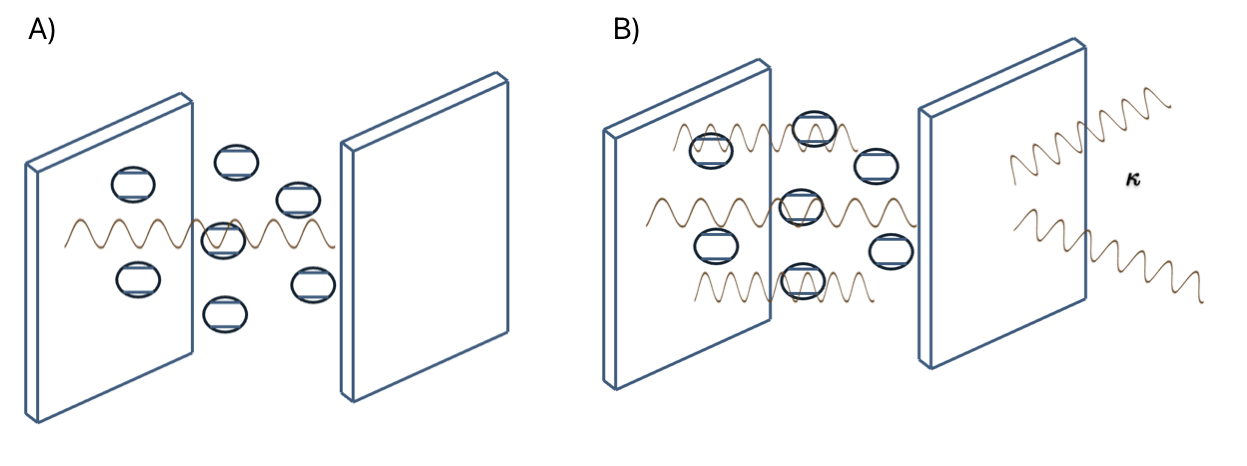
\includegraphics[width=0.9\linewidth]{Images/cavity1.png}
    \caption{Ilustración del modelo de Dicke. 
A) \( N \) átomos de dos niveles interactúan con un único modo electromagnético. 
B) \( N \) átomos interactúan con múltiples modos, incorporando bombeo y disipación \( \kappa \).}
    \label{Figure Cavity}
\end{figure}

La primera observación experimental de la transición superradiante fue realizada por Baumann et al.~\cite{Baumann11} acoplando un condensado de Bose–Einstein (BEC) a una cavidad óptica abierta. Este experimento reveló la ruptura espontánea de simetría durante la transición, mostrando cómo las fluctuaciones cuánticas y efectos disipativos compiten en regímenes fuera del equilibrio~\cite{Baumann10}. Experimentos posteriores con BEC en cavidades ópticas demostraron que la transición superradiante puede mantenerse en régimen no térmico~\cite{Baumann10,Klinder15}, mientras que en circuitos QED se observaron dinámicas colectivas estacionarias inducidas por disipación~\cite{Blais2021}. Estos resultados establecieron la disipación como elemento activo para generar y estabilizar orden cuántico colectivo.

Los sistemas optomecánicos~\cite{debnath2015} y los qubits superconductores~\cite{Lamata2017} han emergido como plataformas experimentales clave. Los primeros permiten estudiar acoplamientos entre modos ópticos y mecánicos, mientras que los segundos ofrecen control preciso sobre parámetros fundamentales, facilitando la exploración experimental de los modelos de Rabi y Dicke~\cite{Mezzacapo14} y su interacción con el entorno~\cite{hwang2018,Lo2021}.

Recientemente, el modelo de Dicke multimodo en regímenes fuera de equilibrio ha mostrado comportamientos análogos a memorias asociativas, con capacidad de reconocer patrones almacenados~\cite{fiorelli2020}. Más allá del régimen Markoviano, sistemas no-Markovianos como los átomos gigantes —donde un emisor se acopla al campo en múltiples puntos espaciales— introducen retardos y correlaciones temporales que permiten simular interacciones con memoria~\cite{kockum2019,guo2020}. Estas configuraciones consolidan el \textit{reservoir engineering} como técnica para diseñar entornos que protegen o inducen coherencia, estabilizando estados coherentes y entrelazados~\cite{poyatos1996,Diehl2008}.


%%%%%%%%%%%%%%%%%%%%%%%%%%%%%%
%%%%%%%%%%%%%%%%%%%%%%%%%%%%%%
\subsection{Conclusión}
%%%%%%%%%%%%%%%%%%%%%%%%%%%%%%
%%%%%%%%%%%%%%%%%%%%%%%%%%%%%%

Este proyecto de investigación doctoral tiene como objetivo principal estudiar sistemáticamente los modelos de Rabi y Dicke en regímenes multimodo y multiqubit, con especial énfasis en sistemas abiertos y fuera de equilibrio. La investigación se estructura progresivamente, comenzando con el modelo de Rabi de dos qubits, sistemas de multifrecuencia bosónica como los átomos gigantes y  avanzando hacia configuraciones colectivas más complejas del modelo de Dicke  donde los efectos no-Markovianos y la estructura  extendida enriquecen sustancialmente la dinámica.


%%%%%%%%%%%%%%%%%%%%%%%%%%%%%%
%%%%%%%%%%%%%%%%%%%%%%%%%%%%%%
\section{Objetivos}
%%%%%%%%%%%%%%%%%%%%%%%%%%%%%%
%%%%%%%%%%%%%%%%%%%%%%%%%%%%%%

El objetivo general de este proyecto es estudiar esquemas fuera de equilibrio en el modelo de Dicke abierto para explorar nuevas fases cuánticas y aplicaciones en el terreno de la información cuántica. 

\begin{itemize}
    \item Comprender el modelo de Dicke multimodo analizando las transiciones de fase superradiante, considerando el caso de 1 o 2 hasta $N$ emisores.
    %%%
    \item Estudiar el modelo de Dicke multimodo abierto y fuera de equilibrio utilizando el formalismo de Keldysh. 
    %%%
    \item Analizar como la competencia entre fluctuaciones cuánticas, disipación y bombeo afecta las propiedades del sistema a diferentes escalas de energía. 
    %%%
    \item Explorar aplicaciones como la posibilidad de cristales de tiempo en el modelo de Dicke multimodo en baños no markovianos, la presencia de memoria a largo plazo y el caso de interacciones entre emisores. 
\end{itemize}



%%%%%%%%%%%%%%%%%%%%%%%%%%%%%%
%%%%%%%%%%%%%%%%%%%%%%%%%%%%%%
\section{Metodología}
%%%%%%%%%%%%%%%%%%%%%%%%%%%%%%
%%%%%%%%%%%%%%%%%%%%%%%%%%%%%%

%%%%%%%%%%%%%%%%%%%%%%%%%%%%%%
%%%%%%%%%%%%%%%%%%%%%%%%%%%%%%
\subsection{Modelo de Rabi de dos qubits con interacciones materiales}
%%%%%%%%%%%%%%%%%%%%%%%%%%%%%%
%%%%%%%%%%%%%%%%%%%%%%%%%%%%%%

Este estudio sistemático del modelo de Rabi de dos qubits con interacciones materiales representa un paso inicial hacia la comprensión de sistemas multiqubit. Implementamos tres aproximaciones  para elucidar cómo la adición de un segundo qubit y las interacciones materiales modifican el espectro energético y los estados del sistema.

%%%%%%%%%%%%%%%%%%%%%%%%%%%%%%
\subsubsection{Diagonalización numérica exacta}
%%%%%%%%%%%%%%%%%%%%%%%%%%%%%%

Como referencia, empleamos diagonalización numérica directa del Hamiltoniano~\eqref{Hamiltoniano de Rabi dos qubits con interacciones}, que proporciona resultados exactos para validar nuestras aproximaciones analíticas. La elección del subespacio simétrico ($j=1$) se justifica por la invariancia del Hamiltoniano bajo permutación de qubits idénticos ($\omega_{01} \approx \omega_{02}$), confinando la dinámica al sector triplete donde los operadores colectivos $\hat{J}_{\alpha}$ capturan completamente el comportamiento del sistema.

En la base producto $|\Psi\rangle = |n\rangle \otimes |j, m\rangle$ con $j=1$, los elementos de matriz son:

\small{ 
\begin{gather}
    \langle n', m' | \hat{H} | n, m \rangle 
    = \omega n\delta_{n',n} + \left(\omega_{0} + \eta_{z}m\right) m\delta_{m',m} 
    + \frac{g}{2}\left( \sqrt{n+1}\delta_{n',n+1} + \sqrt{n}\delta_{n',n-1} \right) \nonumber \\
    \times\left(\sqrt{j(j+1) - m(m+1)}\delta_{m',m+1} + \sqrt{j(j+1) - m(m-1)}\delta_{m',m-1}\right) \nonumber \\
    +\frac{\eta_{x}}{4}\left(\sqrt{j(j+1)-m(m+1)}\sqrt{j(j+1)-(m+1)(m+2)}\delta_{m',m+2} \right. \nonumber \\
    \left. +2\left(j(j+1) - m^{2}\right)\delta_{m',m} \right. \nonumber \\
    \left. +\sqrt{j(j+1) - m(m-1)}\sqrt{j(j+1)-(m-1)(m-2)}\delta_{m',m-2}\right) \label{numerica two qubit}
\end{gather}}   

%%%%%%%%%%%%%%%%%%%%%%%%%%%%%%
\subsubsection{Aproximación adiabática}
%%%%%%%%%%%%%%%%%%%%%%%%%%%%%%

Como primera aproximación analítica, consideramos el límite adiabático ($\omega_0 \rightarrow 0$) donde el oscilador se ajusta instantáneamente a la configuración de los qubits. La transformación $\hat{U} = \exp\left[{\beta(\hat{a}^{\dagger}-\hat{a})}\right]$ genera estados de Fock desplazados que describen el reacomodo del campo para cada configuración de qubits.

Esta aproximación conserva solo acoplamientos entre estados con el mismo número de excitaciones, proporcionando una imagen física intuitiva pero limitada al ignorar efectos de tunelado cuántico.

%%%%%%%%%%%%%%%%%%%%%%%%%%%%%%
\subsubsection{Aproximación de la onda rotante generalizada}
%%%%%%%%%%%%%%%%%%%%%%%%%%%%%%

La Aproximación Generalizada de Onda Rotante (\textit{Generalized Rotating Wave Approximation} o GRWA)~\cite{irish2007,albert2011,yu2012,zhang2015,zhangyu2016,zhangyu2017} extiende el enfoque adiabático reintroduciendo consistentemente el tunelado cuántico mediante la transformación polarónica:

\begin{gather}\label{transformation beta}
    \hat{U} = \exp\left[ \beta\hat{J}_{x}(\hat{a}^{\dagger} - \hat{a}) \right],
\end{gather}

con $\beta=g/\omega$. Esta transformación captura el desplazamiento colectivo del campo electromagnético inducido por los qubits, mientras que la minimización variacional de la energía del estado fundamental incorpora autoconsistentemente los efectos de $\omega_0$.

La GRWA preserva la estructura de bloques manejable de la aproximación adiabática pero incluye correcciones esenciales que permiten describir transiciones entre diferentes números de excitaciones, logrando alta precisión incluso para acoplamientos fuertes.

Esta metodología progresiva —desde la aproximación adiabática simple hasta la GRWA más sofisticada, validadas contra resultados numéricos exactos— establece las bases para extender nuestro análisis a sistemas multiqubit más complejos, donde las interacciones materiales y efectos colectivos juegan roles cruciales en la formación del espectro energético.
 

\clearpage

%%%%%%%%%%%%%%%%%%%%%%%%%%%%%%
%%%%%%%%%%%%%%%%%%%%%%%%%%%%%%
\subsection{Átomos gigantes en guías de onda de arreglo de cavidades}
%%%%%%%%%%%%%%%%%%%%%%%%%%%%%%
%%%%%%%%%%%%%%%%%%%%%%%%%%%%%%

El estudio de átomos gigantes representa una extensión natural de nuestros modelos previos hacia sistemas donde la estructura espacial extendida del emisor introduce efectos no markovianos y de interferencia. A diferencia de los emisores puntuales tradicionales, los átomos gigantes acoplan al campo electromagnético en múltiples puntos espaciales separados, lo que modifica fundamentalmente la dinámica de emisión espontánea.

%%%%%%%%%%%%%%%%%%%%%%%%%%%%%%
\subsubsection{Modelo básico y transformación de Fourier}
%%%%%%%%%%%%%%%%%%%%%%%%%%%%%%

Consideramos un emisor de dos niveles acoplado a un arreglo unidimensional de cavidades, descrito por el Hamiltoniano:

\[H = \delta\sigma^{+}\sigma^{-} + \omega_{0}\sum_{n}a^{\dagger}_{n}a_{n} + \xi\sum_{n}\left(a^{\dagger}_{n+1}a_{n} + a^{\dagger}_{n}a_{n+1}\right) + g_{0}\left(\sigma^{+}a_{0} + \sigma^{-}a^{\dagger}_{0}\right).\]

La clave para resolver este sistema está en aprovechar la invariancia traslacional mediante la transformación de Fourier discreta $a_{k} = N^{-1/2}\sum_{n}e^{ikn}a_{n}$, que diagonaliza la guía de onda y revela la relación de dispersión $\omega_{k} = 2\xi\cos k$. Físicamente, esto significa que en lugar de pensar en cavidades individuales, trabajamos con modos extendidos que se propagan a lo largo de la guía.

%%%%%%%%%%%%%%%%%%%%%%%%%%%%%%
\subsubsection{Función espectral y dinámica no markoviana}
%%%%%%%%%%%%%%%%%%%%%%%%%%%%%%

La función espectral $J(\omega) = \frac{2g_{0}^{2}}{\sqrt{4\xi^{2}-\omega^{2}}}$ captura cómo los diferentes modos de frecuencia $\omega$ contribuyen al acoplamiento. Las singularidades en $\omega = \pm 2\xi$ (bordes de banda) indican el colapso de la aproximación markoviana. Cerca del centro de la banda, $J(\omega)$ es aproximadamente constante y recuperamos la decadencia exponencial tradicional, pero cerca de los bordes la dinámica se vuelve altamente no markoviana.

%%%%%%%%%%%%%%%%%%%%%%%%%%%%%%
\subsubsection{Transformada de Laplace y solución exacta}
%%%%%%%%%%%%%%%%%%%%%%%%%%%%%%

Para ir más allá de la aproximación de Weisskopf-Wigner, empleamos la transformada de Laplace que permite descomponer la solución en contribuciones de estados ligados y de scattering:

\[\alpha(t) = \lim_{\epsilon\to 0}\int_{-\omega_{\max}}^{-\omega_{\min}}\frac{dy}{2\pi}\frac{J(-y)e^{iyt}}{[y+\Delta-iG(-\epsilon+iy)]\,[y+\Delta-iG(\epsilon+iy)]} + \sum_{j}r_{j}e^{-iy_{j}t}.\]

El primer término representa estados de scattering dentro del continuo, mientras que el segundo corresponde a estados ligados (BOC) que persisten en el estado estacionario. Esta descomposición explica físicamente por qué parte de la excitación queda atrapada localmente alrededor del emisor.

%%%%%%%%%%%%%%%%%%%%%%%%%%%%%%
\subsubsection{Extensión a átomos gigantes multimodo}
%%%%%%%%%%%%%%%%%%%%%%%%%%%%%%

La generalización a átomos gigantes que se acoplan en $N_c$ posiciones introduce dependencia espacial explícita:

\[\tilde{g}_k = \frac{g_0}{N_c\sqrt{N}} \frac{\sin(kdN_c/2)}{\sin(kd/2)}.\]

La función espectral efectiva $J_{\text{eff}}(\omega) = J(\omega) \mathcal{G}(\omega)$ ahora presenta ceros en frecuencias específicas $\omega_m = 2\xi\cos(\pi(2m+1)/d)$, donde emergen estados ligados dentro del continuo (BIC). Estos BIC surgen de interferencia destructiva que confina fotones entre los puntos de acoplamiento.




\clearpage

%%%%%%%%%%%%%%%%%%%%%%%%%%%%%%
%%%%%%%%%%%%%%%%%%%%%%%%%%%%%%
\subsection{Átomos Gigantes con modos multimodo}%%%%%%%%%%%%%%%%%%%%%%%%%%%%%%
%%%%%%%%%%%%%%%%%%%%%%%%%%%%%%


%%%%%%%%%%%%%%%%%%%%%%%%%%%%%%
%%%%%%%%%%%%%%%%%%%%%%%%%%%%%%
\subsection{Modelo de Dicke multimodal con interacciones materiales}%%%%%%%%%%%%%%%%%%%%%%%%%%%%%%
%%%%%%%%%%%%%%%%%%%%%%%%%%%%%%










En este proyecto, se abordará el estudio de sistemas cuánticos abiertos y fuera de equilibrio. Se iniciará con el modelo de Rabi~\cite{rabi1936}, empleando técnicas  de diagonalización numéricas~\cite{irish2007} y aproximaciones perturbativas, como la transformación del polarón y métodos variacionales~\cite{gonzalez2021}, para sentar las bases conceptuales. A continuación, se avanzará hacia el modelo de Rabi multimodo~\cite{peng2021}. Finalmente, se continuará al modelo de Dicke multimodo, permitiendo el estudio de transiciones de fase disipativas y fenómenos críticos en sistemas abiertos. 

Para abordar el estudio de sistemas de interacción luz-materia en sistemas abiertos y fuera de equilibrio, se empleará la teoría de Keldysh. Esta metodología es particularmente adecuada para sistemas cuánticos con interacciones fuertes, donde coexisten dinámicas coherentes y disipativas~\cite{kamenev2023,rammer2011}. A diferencia de los métodos tradicionales basados en ecuaciones maestras, la teoría de Keldysh permite describir tanto la evolución unitaria como los efectos disipativos, facilitando el análisis de estados estacionarios no térmicos y transiciones de fase en sistemas complejos~\cite{Sieberer2016}.  La formulación de Keldysh extiende la teoría cuántica de campos (\textit{Quantum Field Theory} o QFT) a través de las integrales de camino en el contorno de Keldysh, para calcular funciones de correlación y respuesta en tiempo real, lo que es esencial para comprender la dinámica del sistema y su comportamiento crítico.

Además, se integrará la teoría de renormalización funcional \textit{Functional Renormalization Group} o FRG), basada en la ecuación de Wetterich~\cite{wetterich1993}, para analizar la disipación a diferentes escalas de energía, especialmente en regímenes críticos o durante transiciones de fase. La FRG permitirá una descripción completa del sistema desde escalas microscópicas hasta macroscópicas, capturando efectos no perturbativos y estudiando la competencia entre coherencia y disipación~\cite{angelakis2007}. Esta aproximación será fundamental para investigar fenómenos como la relajación hacia estados estacionarios y la formación de nuevas fases no convencionales.

En el estudio de sistemas cuánticos abiertos, la teoría de sistemas cuánticos disipativos proporciona un enfoque para describir la interacción entre un sistema y su entorno. Bajo la aproximación markoviana, donde se asume que la memoria del baño es despreciable, esta interacción puede modelarse mediante ecuaciones maestras de Lindblad~\cite{breuer2003,Lindblad1976}, las cuales describen la evolución temporal del sistema de manera efectiva. Este enfoque es esencial para comprender la dinámica de sistemas acoplados a baños markovianos, donde la disipación ocurre de manera instantánea y sin correlaciones temporales significativas~\cite{weiss2012}.

Finalmente, se explorará la aparición de memoria a largo plazo en sistemas de Dicke acoplados a baños no markovianos~\cite{zhu2019,lundgren2020,fiorelli2020}. A diferencia de los baños markovianos, donde la disipación es instantánea, los baños no markovianos introducen correlaciones temporales que pueden alterar significativamente la dinámica del sistema~\cite{orazio2016}. Este enfoque permitirá estudiar cómo la memoria a largo plazo influye en la relajación del sistema y en la naturaleza de las transiciones de fase fuera de equilibrio~\cite{lundgren2020}. %En particular, se investigará la formación y estabilidad de cristales de tiempo, fases de la materia que rompen espontáneamente la simetría de traslación temporal, utilizando el modelo de Dicke multimodo como plataforma teórica~\cite{jager2024}.

%Para abordar el estudio de sistemas cuánticos abiertos, fuera de equilibrio con interacciones fuertes con la posibilidad de realizar bombeos, la teoría de Keldysh se ha convertido en una herramienta importante~\cite{kamenev2023,rammer2011}. A diferencia de los métodos tradicionales basados en la formulación de ecuaciones maestras, la teoría de Keldysh proporciona un marco teórico para describir tanto la dinámica coherente como la disipativa en sistemas cuánticos fuera de equilibrio~\cite{Sieberer2016}. Esta teoría se basa en la formulación de integrales de camino en el contorno de Keldysh, que permite tratar de manera sistemática la evolución temporal de sistemas cuánticos abiertos, incluyendo efectos como la disipación.


%La teoría de Keldysh es particularmente útil para estudiar sistemas con un gran número de grados de libertad, como los que aparecen en el Modelo de Dicke~\cite{torres2013,damanet2019}, donde se ha observado que al someter un bombeo externo con disipación se encuentran transiciones de fase fuera de equilibrio que difieren de las observadas en el modelo de Dicke cerrado~\cite{Sieberer2016}.
%Estas transiciones están caracterizadas por exponentes críticos estáticos y dinámicos que reflejan la naturaleza térmica efectiva de las fluctuaciones de baja frecuencia, incluso en ausencia de un baño térmico externo~\cite{torres2013}. 
%Por lo tanto, seria interesante  analizar propiedades críticas y transiciones de fase del modelo de Dicke multimodo abierto, disipativo y con desorden, por ejemplo, la relajación hacia estados estacionarios~\cite{buchhold2013}, el envejecimiento (aging)~\cite{lang2016}, y la formación de fase de no equilibrio~\cite{gilmore1978}. Estos fenómenos son de gran interés tanto desde el punto de vista teórico como experimental, ya que permiten estudiar cómo las fluctuaciones cuánticas y la disipación afectan la evolución temporal del sistema. 
%En particular, se espera que el desorden induzca una dinámica lenta y una distribución amplia de tiempos de relajación, lo que puede llevar a comportamientos de envejecimiento similares a los observados en vidrios de espín clásicos~\cite{buchhold2013}. 
%Además, la presencia de disipación, como la pérdida de fotones en la cavidad, puede modificar significativamente las propiedades espectrales y de correlación del sistema, llevando a la aparición de nuevas fases fuera de equilibrio.


%Utilizando la formulación de Keldysh como marco teórico a sistemas abiertos no toma en cuenta la disipación a diferentes escalas de energía, complicando el análisis, especialmente en transiciones de fase o en regímenes críticos~\cite{Sieberer2016}. La teoría de renormalización funcional (FRG, por sus siglas en inglés) basada en la ecuación de Wetterich~\cite{wetterich1993,Sieberer2016}  proporciona una descripción completa del sistema, desde la escala microscópica hasta la macroscópica, capturando efectos no perturbativos y permitiendo el estudio de la competencia entre coherencia y disipación~\cite{angelakis2007,Sieberer2016}. En este contexto, utilizando FRG, nos permitira analizar las fluctuaciones cuánticas y la disipación a diferentes escalas de energía, especialmente en las transiciones de fase al modelo de Dicke multimodo. 


%Por último, uno de los fenómenos de los sistemas de Dicke fuera de equilibrio es la aparición de memoria a largo plazo~\cite{zhu2019,lundgren2020,fiorelli2020}, un fenómeno que surge cuando el sistema está acoplado a baños no markovianos. A diferencia de los baños markovianos, donde la disipación es instantánea y no depende de la historia del sistema, los baños no markovianos introducen correlaciones temporales que pueden alterar drásticamente la dinámica del sistema~\cite{orazio2016}. Este tipo de memoria a largo plazo no solo afecta la relajación del sistema hacia un estado estacionario, sino que también puede influir en la naturaleza de las transiciones de fase~\cite{lundgren2020}. En particular, R. Lundgren en el 2020~\cite{lundgren2020} exploró cómo la interacción entre baños markovianos y no markovianos en sistemas de Dicke puede llevar a transiciones de fase clásicas fuera de equilibrio, donde los exponentes críticos dependen de la densidad espectral del baño no markoviano. Una de las transiciones de fase involucradas en sistemas de no equilibrio son los cristales de tiempo~\cite{zhu2019}. Los cristales de tiempo son fases de la materia que rompen espontáneamente la simetría de traslación temporal, exhibiendo un comportamiento periódico en el tiempo incluso en ausencia de un campo externo periódico~\cite{jager2024}. En particular, los sistemas de Dicke fuera de equilibrio representan una plataforma ideal para estudiar la formación y estabilidad de cristales de tiempo.

%B. Zhu en el 2019~\cite{zhu2019}, investigo la estabilidad de los cristales de tiempo en el modelo de Dicke. En su trabajo, demuestran que el comportamiento de cristal de tiempo puede persistir incluso en presencia de interacciones de corto alcance que rompen la naturaleza colectiva del modelo de Dicke tradicional. Además,  identifican que la disipación juega un papel crucial en la estabilización de estos cristales de tiempo, actuando como un mecanismo de enfriamiento que contrarresta el calentamiento inducido por el bombeo periódico al sistema. En este contexto, uno de los objetivos de esta investigación es explorar la formación de cristales de tiempo en sistemas de Dicke multimodo fuera de equilibrio.







%%%%%%%%%%%%%%%%%%%%%%%%%%%%%%
%%%%%%%%%%%%%%%%%%%%%%%%%%%%%%
\section{Resultados Esperados}
%%%%%%%%%%%%%%%%%%%%%%%%%%%%%%
%%%%%%%%%%%%%%%%%%%%%%%%%%%%%%







%%%%%%%%%%%%%%%%%%%%%%%%%%%%%%
%%%%%%%%%%%%%%%%%%%%%%%%%%%%%%
\section{Avances}
%%%%%%%%%%%%%%%%%%%%%%%%%%%%%%
%%%%%%%%%%%%%%%%%%%%%%%%%%%%%%






%%%%%%%%%%%%%%%%%%%%%%%%%%%%%%
%%%%%%%%%%%%%%%%%%%%%%%%%%%%%%
\section{Bibliografía}
%%%%%%%%%%%%%%%%%%%%%%%%%%%%%%
%%%%%%%%%%%%%%%%%%%%%%%%%%%%%%

\printbibliography[heading=none]

\section{Calendario}





\clearpage


\section{Objetivos}

El objetivo general de este proyecto es estudiar esquemas fuera de equilibrio en el modelo de Dicke abierto para explorar nuevas fases cuánticas y aplicaciones en el terreno de la información cuántica. 

\begin{itemize}
    \item Comprender el modelo de Dicke multimodo analizando las transiciones de fase superradiante, considerando el caso de 1 o 2 hasta $N$ emisores.
    %%%
    \item Estudiar el modelo de Dicke multimodo abierto y fuera de equilibrio utilizando el formalismo de Keldysh. 
    %%%
    \item Analizar como la competencia entre fluctuaciones cuánticas, disipación y bombeo afecta las propiedades del sistema a diferentes escalas de energía. 
    %%%
    \item Explorar aplicaciones como la posibilidad de cristales de tiempo en el modelo de Dicke multimodo en baños no markovianos, la presencia de memoria a largo plazo y el caso de interacciones entre emisores. 
\end{itemize}


%%%%%%%%%%%%%%%%%%%%%%%%%%%%%%
%%%%%%%%%%%%%%%%%%%%%%%%%%%%%%

%%%%%%%%%%%%%%%%%%%%%%%%%%%%%%
%%%%%%%%%%%%%%%%%%%%%%%%%%%%%%
\section{Metodología y/o Desarrollo del Tema}
%\textcolor{red}{[Aprox. 5 pp.]}
%%%%%%%%%%%%%%%%%%%%%%%%%%%%%%
%%%%%%%%%%%%%%%%%%%%%%%%%%%%%%

En este proyecto, se abordará el estudio de sistemas cuánticos abiertos y fuera de equilibrio. Se iniciará con el modelo de Rabi~\cite{rabi1936}, empleando técnicas  de diagonalización numéricas~\cite{irish2007} y aproximaciones perturbativas, como la transformación del polarón y métodos variacionales~\cite{gonzalez2021}, para sentar las bases conceptuales. A continuación, se avanzará hacia el modelo de Rabi multimodo~\cite{peng2021}. Finalmente, se continuará al modelo de Dicke multimodo, permitiendo el estudio de transiciones de fase disipativas y fenómenos críticos en sistemas abiertos. 

Para abordar el estudio de sistemas de interacción luz-materia en sistemas abiertos y fuera de equilibrio, se empleará la teoría de Keldysh. Esta metodología es particularmente adecuada para sistemas cuánticos con interacciones fuertes, donde coexisten dinámicas coherentes y disipativas~\cite{kamenev2023,rammer2011}. A diferencia de los métodos tradicionales basados en ecuaciones maestras, la teoría de Keldysh permite describir tanto la evolución unitaria como los efectos disipativos, facilitando el análisis de estados estacionarios no térmicos y transiciones de fase en sistemas complejos~\cite{Sieberer2016}.  La formulación de Keldysh extiende la teoría cuántica de campos (\textit{Quantum Field Theory} o QFT) a través de las integrales de camino en el contorno de Keldysh, para calcular funciones de correlación y respuesta en tiempo real, lo que es esencial para comprender la dinámica del sistema y su comportamiento crítico.

Además, se integrará la teoría de renormalización funcional \textit{Functional Renormalization Group} o FRG), basada en la ecuación de Wetterich~\cite{wetterich1993}, para analizar la disipación a diferentes escalas de energía, especialmente en regímenes críticos o durante transiciones de fase. La FRG permitirá una descripción completa del sistema desde escalas microscópicas hasta macroscópicas, capturando efectos no perturbativos y estudiando la competencia entre coherencia y disipación~\cite{angelakis2007}. Esta aproximación será fundamental para investigar fenómenos como la relajación hacia estados estacionarios y la formación de nuevas fases no convencionales.

En el estudio de sistemas cuánticos abiertos, la teoría de sistemas cuánticos disipativos proporciona un enfoque para describir la interacción entre un sistema y su entorno. Bajo la aproximación markoviana, donde se asume que la memoria del baño es despreciable, esta interacción puede modelarse mediante ecuaciones maestras de Lindblad~\cite{breuer2003,Lindblad1976}, las cuales describen la evolución temporal del sistema de manera efectiva. Este enfoque es esencial para comprender la dinámica de sistemas acoplados a baños markovianos, donde la disipación ocurre de manera instantánea y sin correlaciones temporales significativas~\cite{weiss2012}.

Finalmente, se explorará la aparición de memoria a largo plazo en sistemas de Dicke acoplados a baños no markovianos~\cite{zhu2019,lundgren2020,fiorelli2020}. A diferencia de los baños markovianos, donde la disipación es instantánea, los baños no markovianos introducen correlaciones temporales que pueden alterar significativamente la dinámica del sistema~\cite{orazio2016}. Este enfoque permitirá estudiar cómo la memoria a largo plazo influye en la relajación del sistema y en la naturaleza de las transiciones de fase fuera de equilibrio~\cite{lundgren2020}. %En particular, se investigará la formación y estabilidad de cristales de tiempo, fases de la materia que rompen espontáneamente la simetría de traslación temporal, utilizando el modelo de Dicke multimodo como plataforma teórica~\cite{jager2024}.

%Para abordar el estudio de sistemas cuánticos abiertos, fuera de equilibrio con interacciones fuertes con la posibilidad de realizar bombeos, la teoría de Keldysh se ha convertido en una herramienta importante~\cite{kamenev2023,rammer2011}. A diferencia de los métodos tradicionales basados en la formulación de ecuaciones maestras, la teoría de Keldysh proporciona un marco teórico para describir tanto la dinámica coherente como la disipativa en sistemas cuánticos fuera de equilibrio~\cite{Sieberer2016}. Esta teoría se basa en la formulación de integrales de camino en el contorno de Keldysh, que permite tratar de manera sistemática la evolución temporal de sistemas cuánticos abiertos, incluyendo efectos como la disipación.


%La teoría de Keldysh es particularmente útil para estudiar sistemas con un gran número de grados de libertad, como los que aparecen en el Modelo de Dicke~\cite{torres2013,damanet2019}, donde se ha observado que al someter un bombeo externo con disipación se encuentran transiciones de fase fuera de equilibrio que difieren de las observadas en el modelo de Dicke cerrado~\cite{Sieberer2016}.
%Estas transiciones están caracterizadas por exponentes críticos estáticos y dinámicos que reflejan la naturaleza térmica efectiva de las fluctuaciones de baja frecuencia, incluso en ausencia de un baño térmico externo~\cite{torres2013}. 
%Por lo tanto, seria interesante  analizar propiedades críticas y transiciones de fase del modelo de Dicke multimodo abierto, disipativo y con desorden, por ejemplo, la relajación hacia estados estacionarios~\cite{buchhold2013}, el envejecimiento (aging)~\cite{lang2016}, y la formación de fase de no equilibrio~\cite{gilmore1978}. Estos fenómenos son de gran interés tanto desde el punto de vista teórico como experimental, ya que permiten estudiar cómo las fluctuaciones cuánticas y la disipación afectan la evolución temporal del sistema. 
%En particular, se espera que el desorden induzca una dinámica lenta y una distribución amplia de tiempos de relajación, lo que puede llevar a comportamientos de envejecimiento similares a los observados en vidrios de espín clásicos~\cite{buchhold2013}. 
%Además, la presencia de disipación, como la pérdida de fotones en la cavidad, puede modificar significativamente las propiedades espectrales y de correlación del sistema, llevando a la aparición de nuevas fases fuera de equilibrio.


%Utilizando la formulación de Keldysh como marco teórico a sistemas abiertos no toma en cuenta la disipación a diferentes escalas de energía, complicando el análisis, especialmente en transiciones de fase o en regímenes críticos~\cite{Sieberer2016}. La teoría de renormalización funcional (FRG, por sus siglas en inglés) basada en la ecuación de Wetterich~\cite{wetterich1993,Sieberer2016}  proporciona una descripción completa del sistema, desde la escala microscópica hasta la macroscópica, capturando efectos no perturbativos y permitiendo el estudio de la competencia entre coherencia y disipación~\cite{angelakis2007,Sieberer2016}. En este contexto, utilizando FRG, nos permitira analizar las fluctuaciones cuánticas y la disipación a diferentes escalas de energía, especialmente en las transiciones de fase al modelo de Dicke multimodo. 


%Por último, uno de los fenómenos de los sistemas de Dicke fuera de equilibrio es la aparición de memoria a largo plazo~\cite{zhu2019,lundgren2020,fiorelli2020}, un fenómeno que surge cuando el sistema está acoplado a baños no markovianos. A diferencia de los baños markovianos, donde la disipación es instantánea y no depende de la historia del sistema, los baños no markovianos introducen correlaciones temporales que pueden alterar drásticamente la dinámica del sistema~\cite{orazio2016}. Este tipo de memoria a largo plazo no solo afecta la relajación del sistema hacia un estado estacionario, sino que también puede influir en la naturaleza de las transiciones de fase~\cite{lundgren2020}. En particular, R. Lundgren en el 2020~\cite{lundgren2020} exploró cómo la interacción entre baños markovianos y no markovianos en sistemas de Dicke puede llevar a transiciones de fase clásicas fuera de equilibrio, donde los exponentes críticos dependen de la densidad espectral del baño no markoviano. Una de las transiciones de fase involucradas en sistemas de no equilibrio son los cristales de tiempo~\cite{zhu2019}. Los cristales de tiempo son fases de la materia que rompen espontáneamente la simetría de traslación temporal, exhibiendo un comportamiento periódico en el tiempo incluso en ausencia de un campo externo periódico~\cite{jager2024}. En particular, los sistemas de Dicke fuera de equilibrio representan una plataforma ideal para estudiar la formación y estabilidad de cristales de tiempo.

%B. Zhu en el 2019~\cite{zhu2019}, investigo la estabilidad de los cristales de tiempo en el modelo de Dicke. En su trabajo, demuestran que el comportamiento de cristal de tiempo puede persistir incluso en presencia de interacciones de corto alcance que rompen la naturaleza colectiva del modelo de Dicke tradicional. Además,  identifican que la disipación juega un papel crucial en la estabilización de estos cristales de tiempo, actuando como un mecanismo de enfriamiento que contrarresta el calentamiento inducido por el bombeo periódico al sistema. En este contexto, uno de los objetivos de esta investigación es explorar la formación de cristales de tiempo en sistemas de Dicke multimodo fuera de equilibrio.





%%%%%%%%%%%%%%%%%%%%%%%%%%%%%%
%%%%%%%%%%%%%%%%%%%%%%%%%%%%%%
\section{Resultados Esperados}
%\textcolor{red}{[Aprox. 2 pp.]}
%%%%%%%%%%%%%%%%%%%%%%%%%%%%%%
%%%%%%%%%%%%%%%%%%%%%%%%%%%%%%

Se espera que esta investigación aporte avances en la comprensión del modelo de Dicke multimodo en sistemas abiertos y fuera de equilibrio, enfocándose en fenómenos clave como las transiciones de fase superradiantes, la competencia entre modos y los efectos del desorden o interacciones entre emisores. En este análisis, se caracterizará cómo la disipación y la interacción entre modos influyen en las propiedades críticas y la coherencia cuántica del sistema. Los resultados incluirán la identificación de nuevas fases fuera de equilibrio utilizando el formalismo de Keldysh, y la exploración de aplicaciones, como la formación de cristales de tiempo y la implementación de memorias cuánticas con memoria a largo plazo. Estos avances no solo ampliarán el conocimiento teórico en sistemas cuánticos abiertos, sino que también permitirá la exploración de nuevas aplicaciones en el terreno de las tecnologías cuánticas.

%%%%%%%%%%%%%%%%%%%%%%%%%%%%%%
%%%%%%%%%%%%%%%%%%%%%%%%%%%%%%
\section{Cronología}
%%%%%%%%%%%%%%%%%%%%%%%%%%%%%%
%%%%%%%%%%%%%%%%%%%%%%%%%%%%%%

De acuerdo con el plan de estudios del  Posgrado en Ciencias (Física):

\noindent El cronograma de la estancia está dividido en 12 trimestres. Dentro de cada trimestre, semanalmente, se entregarán avances del proyecto así como la aclaración de dudas y corrección de errores (en el caso que se presente). 

\begin{figure}[H]
    \centering
    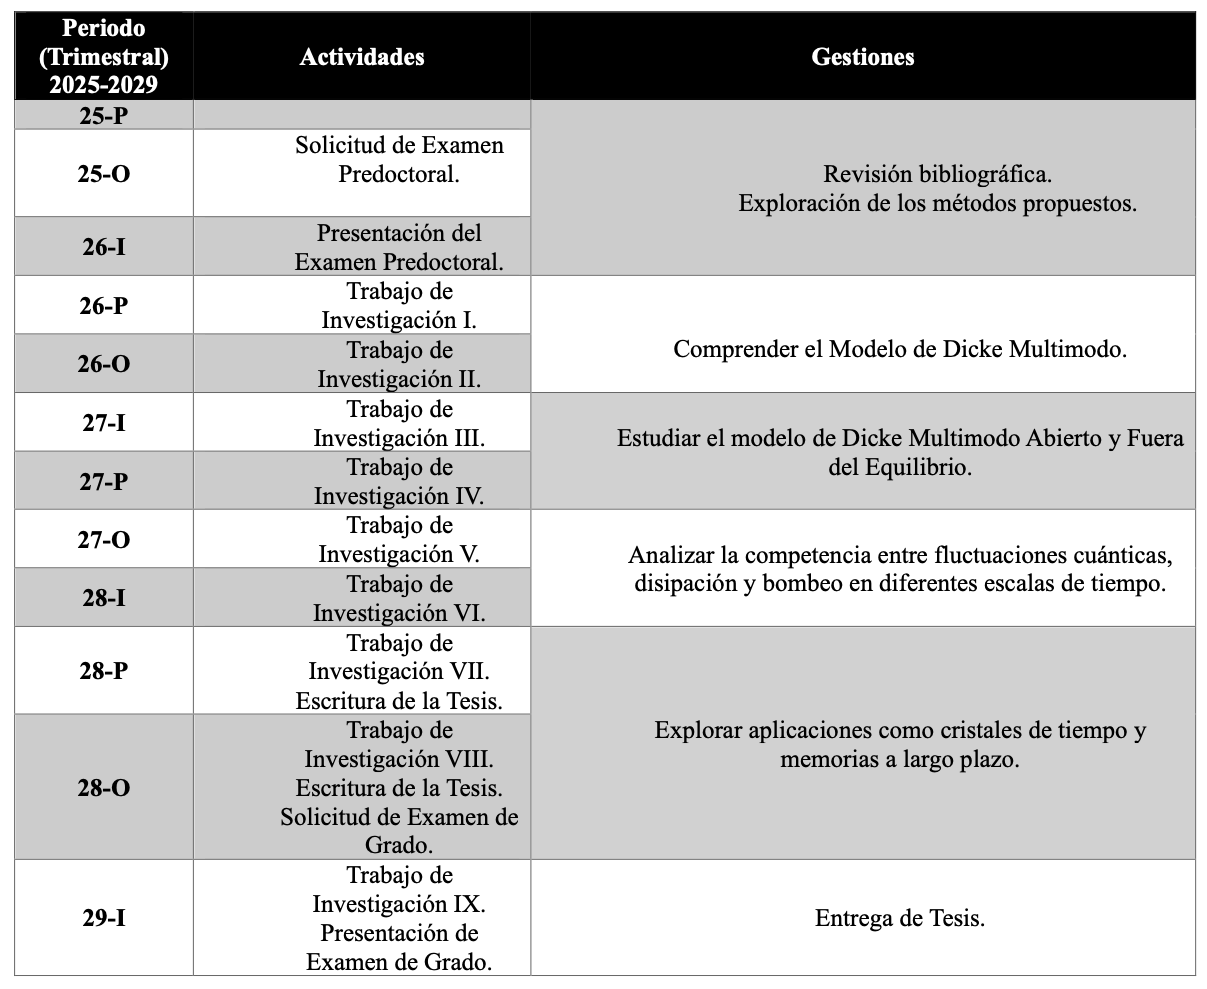
\includegraphics[width=1\linewidth]{Images/Tabla Cronologia.png}

\end{figure}

\begin{comment}
\noindent\textbf{Trimestre I-III}:
%%%
\begin{itemize}
    %%%
    \item  Extensión del Modelo de Dicke a sistemas multimodos. 
    %%%
    \begin{itemize}
        \item Estudiar el Modelo de Dicke, donde los átomos interactuan con múltiples modos fotónicos. 
        %%%
        \item Analizar las transiciones de fase superradiante y sus propiedades en sistemas multimodo. 
        %%%
    \end{itemize}
    %%%
    \item Efectos de desorden en el Modelo de Dicke. 
    %%%
    \begin{itemize}
        \item Investigar como el desorden en acoplamientos átomo-fotón afecta las transiciones de fase superradiantes. 
        %%% 
    \end{itemize}
\end{itemize}
%%%
\textbf{Trimestre IV-VI}:
%%%
\begin{itemize}
    %%%
    \item Extensión del Modelo de Dicke con disipación
    %%%
    \begin{itemize}
        \item Estudiar el modelo de Dicke en presencia de disipación utilizando la teoría de Keldysh. 
        %%%
        \item Analizar como la disipación afecta las transiciones de fase superradiantes y sus propiedades
        %%%
     \end{itemize}
    %%%
    \item  Dinámica de sistemas fuera de equilibrio en el Modelo de Dicke
    %%%
    \begin{itemize}
    %%%
        \item Utilizar el formalismo de Keldysh para estudiar la dinámica de relajación con desorden y disipación 
        %%%
        \item Explorar como las fluctuaciones cuánticas afecta la evolución temporal del sistema 
    \end{itemize}
\end{itemize}
%%%
\textbf{Trimestre VII-IX}:
\begin{itemize}
%%%
    \item Modelo de Dicke de dos fotones y Modelo de Rabi 
    %%%
    \begin{itemize}
    %%%
        \item Estudiar el Modelo de Dicke de dos fotones y Rabi en presencia de disipación. 
        %%%
        \item Analizar como la disipación afecta las transiciones de fase superradiantes y sus propiedades. 
    \end{itemize}
    %%%
    \item Teoría de renormalización funcional para sistemas abiertos.
    %%%
    \begin{itemize}
        \item Aplicar la teoría de renormalización funcional a sistemas abiertos. 
        %%%
        \item Estudiar como las fluctuaciones cuánticas y la disipación afectan las propiedades del sistema a diferentes escalas de energía. 
    \end{itemize}
\end{itemize}
%%%
\textbf{Trimestre X-XII}:
%%%
\begin{itemize} 
    %%%
    \item Aplicaciones en sistemas de Dicke fuera de equilibrio
    %%%
    \begin{itemize}
        \item Estudiar la posibilidad de cristales de tiempo en sistemas de Dicke acoplados a baños no markovianos. 
        %%%
        \item Explorar como la memoria a largo plazo afecta a la formación de estos estados. 
    \end{itemize}
\end{itemize}

\end{comment}







%%%%%%%%%%%%%%%%%%%%%%%%%%%%%%
%%%%%%%%%%%%%%%%%%%%%%%%%%%%%%
\section{Bibliografía}

%%%%%%%%%%%%%%%%%%%%%%%%%%%%%%
%%%%%%%%%%%%%%%%%%%%%%%%%%%%%%

\end{document}
